\chapter{Implementation Roadmap}
\label{chap:implementation-roadmap}

\section*{Integration with existing chapters}
\addcontentsline{toc}{section}{Integration with existing chapters}

This chapter extends the project roadmap in Chapter~\ref{sec:sim-roadmap} with 
enterprise deployment phases:

\begin{itemize}
  \item \textbf{Chapter~\ref{sec:sim-roadmap}} (Project Roadmap): The v1.2 
    milestones (M01--M07) defined there are \emph{prerequisites} for this 
    enterprise roadmap. Phase 1 here begins only after M07 (v1.2 tag) is complete.
  \item \textbf{Chapter~\ref{ch:agent-impl}} (Agent Instructions): Tasks S1--S6 
    in that chapter deliver the technical foundation; this roadmap adds the 
    business governance wrapper (BR-1.x through BR-5.x).
  \item \textbf{Chapter~\ref{chap:business-requirements}} (Business Requirements): 
    Each phase in this roadmap addresses specific BR requirements, as shown in 
    \cref{tab:req-by-phase}.
  \item \textbf{Figure~\ref{fig:sim-dependency-graph}} (Dependency Graph): This 
    roadmap extends the dependency graph with enterprise deployment nodes that 
    follow the Could (C01) milestone.
\end{itemize}

\noindent
Like Chapter~\ref{sec:sim-roadmap}, this roadmap expresses \emph{sequence} and 
\emph{dependency}, not calendar dates. The phases are ordered by prerequisite 
relationships and risk, not by time estimates.

\section*{Scope of this chapter}
\addcontentsline{toc}{section}{Scope of this chapter}

This chapter defines the phased implementation roadmap for enterprise deployment
of the Simula synthetic data framework. The roadmap is organized into three
sequential phases, each building upon the capabilities established in the
previous phase. Phases are sequenced by dependency and risk, not by time
estimates.

\section*{Relationship to Chapter~\ref{sec:sim-roadmap} Milestones}
\addcontentsline{toc}{section}{Relationship to Project Milestones}

This enterprise roadmap extends the technical milestones defined in 
Chapter~\ref{sec:sim-roadmap}. The mapping below clarifies which project
milestones are addressed by each enterprise phase:

\begin{table}[htbp]
\centering
\caption{Mapping of Project Milestones (Ch.~\ref{sec:sim-roadmap}) to Enterprise Phases (Ch.~\ref{chap:implementation-roadmap})}
\label{tab:milestone-to-phase}
\footnotesize
\begin{tabularx}{\textwidth}{@{}l l l X@{}}
\toprule
\textbf{Milestone} & \textbf{MoSCoW} & \textbf{Phase} & \textbf{Relationship} \\
\midrule
M01--M07 & Must & \textit{Prerequisite} & v1.2 technical foundation; completes before Phase 1 \\
S01--S03 & Should & Phase 1 & Addressed during capability building \\
C01--C02 & Could & Phase 2 & Addressed during scaled deployment \\
M08 (Business Case Refresh) & Must & Phase 1 Exit & Gate check before Phase 2 \\
\bottomrule
\end{tabularx}
\end{table}

\noindent
\textbf{Key Relationships:}
\begin{itemize}
  \item \textbf{Phase 1} corresponds to completing the ``Should'' milestones (S01--S03)
        plus establishing enterprise governance (BR-3.x, BR-4.x requirements).
  \item \textbf{Phase 2} corresponds to completing the ``Could'' milestones (C01--C02)
        plus achieving production scale (BR-2.x requirements).
  \item \textbf{Phase 3} represents continuous operations beyond the initial roadmap,
        addressing long-term optimization and BR-5.x requirements.
  \item \textbf{M08 (Business Case Refresh)} from Chapter~\ref{sec:sim-roadmap} serves
        as the Phase 1 exit gate, requiring documented ROI before Phase 2 investment.
\end{itemize}

\subsection*{Typical Duration Estimates}

While this roadmap does not commit to calendar dates, the following are typical
duration ranges assuming dedicated resources:

\begin{table}[htbp]
\centering
\caption{Typical Phase Durations (Resource-Dependent)}
\label{tab:typical-durations}
\footnotesize
\begin{tabular}{@{}l l l@{}}
\toprule
\textbf{Phase} & \textbf{Typical Duration} & \textbf{Assumptions} \\
\midrule
Phase 1 & 2--4 months & 3 FTE engineers, infrastructure ready \\
Phase 2 & 3--6 months & Pilot success, production resources allocated \\
Phase 3 & Ongoing & Operational team in place \\
\bottomrule
\end{tabular}
\end{table}

\noindent
These estimates are indicative only. Actual duration depends on organizational
readiness, infrastructure availability, and competing priorities.

\section{Roadmap Overview}

\begin{figure}[htbp]
\centering
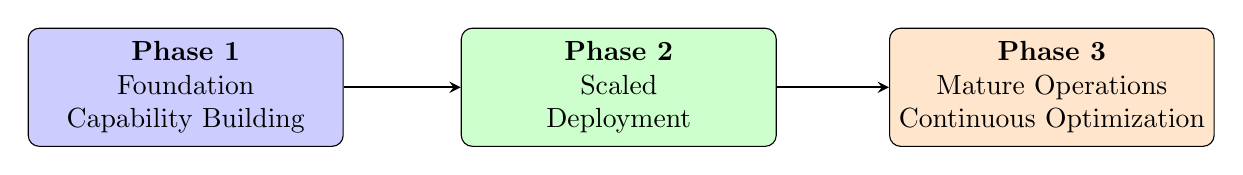
\begin{tikzpicture}[
    phase/.style={rectangle, draw, rounded corners, minimum width=4cm, minimum height=1.5cm, align=center},
    arrow/.style={->, thick, >=stealth}
]
    \node[phase, fill=blue!20] (p1) at (0,0) {\textbf{Phase 1}\\Foundation\\Capability Building};
    \node[phase, fill=green!20] (p2) at (5.5,0) {\textbf{Phase 2}\\Scaled\\Deployment};
    \node[phase, fill=orange!20] (p3) at (11,0) {\textbf{Phase 3}\\Mature Operations\\Continuous Optimization};
    
    \draw[arrow] (p1) -- (p2);
    \draw[arrow] (p2) -- (p3);
\end{tikzpicture}
\caption{Simula implementation phases.}
\label{fig:phases}
\end{figure}

\subsection{Phase Dependencies}

Each phase has explicit entry criteria that must be satisfied before proceeding:

\begin{table}[htbp]
\centering
\caption{Phase entry criteria.}
\label{tab:phase-entry}
\footnotesize
\begin{tabularx}{\textwidth}{@{}l X@{}}
\toprule
\textbf{Phase} & \textbf{Entry Criteria} \\
\midrule
Phase 1 & Executive sponsorship, initial use case identified \\
Phase 2 & Phase 1 complete, pilot success criteria met, production infrastructure available \\
Phase 3 & Phase 2 complete, multiple use cases in production, operational team trained \\
\bottomrule
\end{tabularx}
\end{table}


\section{Phase 1: Foundation Capability Building}

Phase 1 establishes the foundational capabilities required for Simula deployment,
focusing on a single high-value use case to validate the approach before scaling.

\subsection{Phase 1 Objectives}

\begin{enumerate}
  \item Establish organizational readiness and governance integration
  \item Deploy core Simula pipeline for pilot use case
  \item Validate quality and utility through downstream evaluation
  \item Build internal expertise and operational procedures
\end{enumerate}

\subsection{Phase 1 Deliverables}

\subsubsection{1.1 Use Case Definition and Value-Risk Assessment}

\begin{tcolorbox}[colback=blue!5,colframe=blue!70,title=1.1 Use Case and Risk Assessment]
\textbf{Requirements Addressed}: BR-1.1, BR-1.2

\textbf{Activities}:
\begin{itemize}
  \item Identify and document pilot use case with clear business objective
  \item Conduct structured value-risk assessment
  \item Define success criteria and measurement approach
  \item Obtain executive sponsor approval
\end{itemize}

\textbf{Deliverables}:
\begin{itemize}
  \item Use case specification document
  \item Value-risk assessment matrix
  \item Success criteria definition
  \item Executive sign-off
\end{itemize}

\textbf{Exit Criteria}: Documented use case with approved risk assessment
\end{tcolorbox}

\subsubsection{1.2 Cross-Functional Team Assembly}

\begin{tcolorbox}[colback=blue!5,colframe=blue!70,title=1.2 Team Organization]
\textbf{Requirements Addressed}: BR-1.4

\textbf{Activities}:
\begin{itemize}
  \item Identify and assign team members across functions
  \item Establish communication cadence and escalation paths
  \item Define decision-making authority matrix
  \item Conduct initial training on Simula concepts
\end{itemize}

\textbf{Deliverables}:
\begin{itemize}
  \item Team charter with named individuals
  \item RACI matrix for Simula activities
  \item Communication plan
  \item Training completion records
\end{itemize}

\textbf{Exit Criteria}: Functional team with clear roles and responsibilities
\end{tcolorbox}

\subsubsection{1.3 Governance Framework Integration}

\begin{tcolorbox}[colback=blue!5,colframe=blue!70,title=1.3 Governance Integration]
\textbf{Requirements Addressed}: BR-1.3

\textbf{Activities}:
\begin{itemize}
  \item Map synthetic data activities to existing governance frameworks
  \item Draft synthetic data policies and procedures
  \item Configure approval workflows in existing tools
  \item Update stakeholder training materials
\end{itemize}

\textbf{Deliverables}:
\begin{itemize}
  \item Synthetic data policy document
  \item Updated governance framework documentation
  \item Configured approval workflows
  \item Training materials
\end{itemize}

\textbf{SAP Integration}: Configure SAP GRC for policy management

\textbf{Exit Criteria}: Governance policies documented and integrated
\end{tcolorbox}

\subsubsection{1.4 Domain Taxonomy Construction}

\begin{tcolorbox}[colback=blue!5,colframe=blue!70,title=1.4 Taxonomy Development]
\textbf{Requirements Addressed}: BR-2.1

\textbf{Activities}:
\begin{itemize}
  \item Extract domain factors from pilot use case schema
  \item Generate initial taxonomies using Simula taxonomy builder
  \item Conduct domain expert review and validation
  \item Establish taxonomy version control
\end{itemize}

\textbf{Deliverables}:
\begin{itemize}
  \item Domain taxonomy artifacts (JSON/YAML)
  \item Expert validation sign-off
  \item Coverage gap analysis report
  \item Taxonomy versioning repository
\end{itemize}

\textbf{SAP Integration}: Store taxonomies in SAP HANA Cloud

\textbf{Exit Criteria}: Validated taxonomy with expert approval
\end{tcolorbox}

\subsubsection{1.5 Metadata and Provenance Infrastructure}

\begin{tcolorbox}[colback=blue!5,colframe=blue!70,title=1.5 Provenance System]
\textbf{Requirements Addressed}: BR-2.4

\textbf{Activities}:
\begin{itemize}
  \item Design metadata schema for generation provenance
  \item Implement automatic metadata capture in pipeline
  \item Configure tamper-evident storage
  \item Build metadata query interface
\end{itemize}

\textbf{Deliverables}:
\begin{itemize}
  \item Metadata schema definition
  \item Provenance capture implementation
  \item Storage configuration
  \item Query interface
\end{itemize}

\textbf{SAP Integration}: Utilize SAP HANA Cloud for metadata storage with
hash-chained integrity

\textbf{Exit Criteria}: Automated provenance capture operational
\end{tcolorbox}

\subsubsection{1.6 Quality Assessment Pipeline}

\begin{tcolorbox}[colback=blue!5,colframe=blue!70,title=1.6 Quality Evaluation]
\textbf{Requirements Addressed}: BR-3.1, BR-3.2

\textbf{Activities}:
\begin{itemize}
  \item Implement intrinsic quality metrics (coverage, diversity, complexity)
  \item Build automated quality report generation
  \item Configure downstream validation pipeline (TSTR)
  \item Establish quality thresholds and gates
\end{itemize}

\textbf{Deliverables}:
\begin{itemize}
  \item Quality evaluation module
  \item Automated report templates
  \item TSTR pipeline configuration
  \item Quality gate definitions
\end{itemize}

\textbf{SAP Integration}: Execute validation via SAP AI Core

\textbf{Exit Criteria}: Quality pipeline generating actionable reports
\end{tcolorbox}

\subsection{Phase 1 Exit Criteria}

Phase 1 is complete when:
\begin{itemize}
  \item[\checkmark] Pilot use case successfully generates synthetic dataset
  \item[\checkmark] Downstream model trained on synthetic data meets quality gate
  \item[\checkmark] Governance policies documented and approved
  \item[\checkmark] Provenance and quality systems operational
  \item[\checkmark] Team trained and operational procedures documented
\end{itemize}


\section{Phase 2: Scaled Deployment}

Phase 2 scales Simula capabilities to production usage with multiple use cases,
implementing user-facing interfaces and comprehensive compliance mechanisms.

\subsection{Phase 2 Objectives}

\begin{enumerate}
  \item Enable self-service generation for business users
  \item Implement comprehensive privacy and bias controls
  \item Deploy production access control and audit systems
  \item Integrate with enterprise ML pipelines
\end{enumerate}

\subsection{Phase 2 Deliverables}

\subsubsection{2.1 Parameter Configuration Interface}

\begin{tcolorbox}[colback=green!5,colframe=green!70,title=2.1 User Configuration Interface]
\textbf{Requirements Addressed}: BR-2.2

\textbf{Activities}:
\begin{itemize}
  \item Design visual configuration interface
  \item Implement parameter validation and constraint checking
  \item Build preview mode for distribution estimation
  \item Create configuration templates for common scenarios
\end{itemize}

\textbf{Deliverables}:
\begin{itemize}
  \item Web-based configuration UI
  \item Parameter validation logic
  \item Preview visualization
  \item Template library
\end{itemize}

\textbf{SAP Integration}: Build using SAP Build Apps; store configurations in
SAP HANA Cloud

\textbf{Exit Criteria}: Business users can configure and launch generation tasks
\end{tcolorbox}

\subsubsection{2.2 Privacy Risk Assessment System}

\begin{tcolorbox}[colback=green!5,colframe=green!70,title=2.2 Privacy Controls]
\textbf{Requirements Addressed}: BR-3.3

\textbf{Activities}:
\begin{itemize}
  \item Implement membership inference attack testing
  \item Build similarity scanning against reference datasets
  \item Configure privacy risk scoring and thresholds
  \item Design remediation workflow for high-risk samples
\end{itemize}

\textbf{Deliverables}:
\begin{itemize}
  \item Privacy risk evaluation module
  \item Similarity scanner
  \item Risk scoring dashboard
  \item Remediation workflow
\end{itemize}

\textbf{SAP Integration}: Integrate with SAP Data Privacy Integration

\textbf{Exit Criteria}: Automated privacy screening on all generated datasets
\end{tcolorbox}

\subsubsection{2.3 Bias Detection and Mitigation}

\begin{tcolorbox}[colback=green!5,colframe=green!70,title=2.3 Bias Controls]
\textbf{Requirements Addressed}: BR-3.4

\textbf{Activities}:
\begin{itemize}
  \item Implement distribution analysis on sensitive attributes
  \item Build fairness metric computation
  \item Design bias mitigation recommendations
  \item Create bias audit trail
\end{itemize}

\textbf{Deliverables}:
\begin{itemize}
  \item Bias detection module
  \item Fairness metrics dashboard
  \item Mitigation recommendation engine
  \item Audit trail storage
\end{itemize}

\textbf{Exit Criteria}: Bias screening integrated into generation pipeline
\end{tcolorbox}

\subsubsection{2.4 Access Control and Permissions}

\begin{tcolorbox}[colback=green!5,colframe=green!70,title=2.4 RBAC Implementation]
\textbf{Requirements Addressed}: BR-4.1

\textbf{Activities}:
\begin{itemize}
  \item Configure role-based access control
  \item Implement dataset access approval workflows
  \item Define domain-specific access policies
  \item Enable comprehensive access logging
\end{itemize}

\textbf{Deliverables}:
\begin{itemize}
  \item RBAC configuration
  \item Approval workflow
  \item Access policies
  \item Audit log configuration
\end{itemize}

\textbf{SAP Integration}: Leverage SAP Cloud Identity Services and XSUAA

\textbf{Exit Criteria}: Production access controls operational
\end{tcolorbox}

\subsubsection{2.5 ML Pipeline Integration}

\begin{tcolorbox}[colback=green!5,colframe=green!70,title=2.5 MLOps Integration]
\textbf{Requirements Addressed}: BR-5.1

\textbf{Activities}:
\begin{itemize}
  \item Implement REST API for generation task management
  \item Build SAP AI Core integration
  \item Configure webhook notifications
  \item Enable artifact registration in ML pipelines
\end{itemize}

\textbf{Deliverables}:
\begin{itemize}
  \item Generation task API
  \item SAP AI Core connector
  \item Webhook configuration
  \item Pipeline integration documentation
\end{itemize}

\textbf{SAP Integration}: Primary integration with SAP AI Core MLOps

\textbf{Exit Criteria}: Simula integrated into production ML pipelines
\end{tcolorbox}

\subsubsection{2.6 Audit Logging System}

\begin{tcolorbox}[colback=green!5,colframe=green!70,title=2.6 Audit Trail]
\textbf{Requirements Addressed}: BR-4.3

\textbf{Activities}:
\begin{itemize}
  \item Deploy tamper-evident audit log storage
  \item Implement comprehensive event logging
  \item Build query interface for investigations
  \item Configure retention policies
\end{itemize}

\textbf{Deliverables}:
\begin{itemize}
  \item Audit log storage
  \item Event logging implementation
  \item Query interface
  \item Retention configuration
\end{itemize}

\textbf{SAP Integration}: Utilize SAP Audit Log Service

\textbf{Exit Criteria}: Complete audit trail for all Simula activities
\end{tcolorbox}

\subsection{Phase 2 Exit Criteria}

Phase 2 is complete when:
\begin{itemize}
  \item[\checkmark] Multiple use cases deployed in production
  \item[\checkmark] Business users can self-service generation tasks
  \item[\checkmark] Privacy and bias controls operational
  \item[\checkmark] Access control and audit systems production-ready
  \item[\checkmark] Integration with enterprise ML pipelines complete
\end{itemize}


\section{Phase 3: Mature Operations and Continuous Optimization}

Phase 3 establishes mature operational capabilities with continuous monitoring,
optimization, and advanced features for long-term sustainability.

\subsection{Phase 3 Objectives}

\begin{enumerate}
  \item Implement continuous quality monitoring and drift detection
  \item Complete regulatory compliance and transparency requirements
  \item Establish incident response capabilities
  \item Optimize costs and enable advanced features
\end{enumerate}

\subsection{Phase 3 Deliverables}

\subsubsection{3.1 Continuous Monitoring and Drift Detection}

\begin{tcolorbox}[colback=orange!5,colframe=orange!70,title=3.1 Quality Monitoring]
\textbf{Requirements Addressed}: BR-3.5

\textbf{Activities}:
\begin{itemize}
  \item Implement scheduled quality sampling jobs
  \item Build drift detection with statistical testing
  \item Configure alerts for threshold breaches
  \item Enable automated remediation triggers
\end{itemize}

\textbf{Deliverables}:
\begin{itemize}
  \item Monitoring job scheduler
  \item Drift detection module
  \item Alert configuration
  \item Remediation automation
\end{itemize}

\textbf{SAP Integration}: Configure via SAP AI Core; alerts via SAP Alert
Notification Service

\textbf{Exit Criteria}: Continuous monitoring operational with alert coverage
\end{tcolorbox}

\subsubsection{3.2 Regulatory Compliance Completion}

\begin{tcolorbox}[colback=orange!5,colframe=orange!70,title=3.2 Compliance Framework]
\textbf{Requirements Addressed}: BR-4.2

\textbf{Activities}:
\begin{itemize}
  \item Document compliance position for each applicable regulation
  \item Obtain legal review sign-off
  \item Establish regulatory change monitoring
  \item Implement jurisdiction-specific variations
\end{itemize}

\textbf{Deliverables}:
\begin{itemize}
  \item Compliance documentation
  \item Legal sign-off records
  \item Regulatory monitoring process
  \item Jurisdiction policy matrix
\end{itemize}

\textbf{SAP Integration}: Integrate with SAP GRC for regulatory tracking

\textbf{Exit Criteria}: Documented compliance for all applicable regulations
\end{tcolorbox}

\subsubsection{3.3 Transparency and Explainability}

\begin{tcolorbox}[colback=orange!5,colframe=orange!70,title=3.3 External Transparency]
\textbf{Requirements Addressed}: BR-4.4

\textbf{Activities}:
\begin{itemize}
  \item Create synthetic data documentation templates
  \item Develop stakeholder communication guidelines
  \item Build model card integration
  \item Prepare FAQ and training materials
\end{itemize}

\textbf{Deliverables}:
\begin{itemize}
  \item Documentation templates
  \item Communication guidelines
  \item Model card integration
  \item FAQ materials
\end{itemize}

\textbf{Exit Criteria}: Transparency materials available for all use cases
\end{tcolorbox}

\subsubsection{3.4 Incident Response Procedures}

\begin{tcolorbox}[colback=orange!5,colframe=orange!70,title=3.4 Incident Management]
\textbf{Requirements Addressed}: BR-4.5

\textbf{Activities}:
\begin{itemize}
  \item Define incident classification and severity matrix
  \item Identify responsible parties for each scenario
  \item Establish escalation and notification paths
  \item Create remediation playbooks
\end{itemize}

\textbf{Deliverables}:
\begin{itemize}
  \item Incident classification matrix
  \item Responsibility assignment
  \item Escalation procedures
  \item Playbooks
\end{itemize}

\textbf{SAP Integration}: Integrate with existing incident management

\textbf{Exit Criteria}: Incident response procedures documented and tested
\end{tcolorbox}

\subsubsection{3.5 Cost and Budget Optimization}

\begin{tcolorbox}[colback=orange!5,colframe=orange!70,title=3.5 Cost Management]
\textbf{Requirements Addressed}: BR-2.3

\textbf{Activities}:
\begin{itemize}
  \item Implement budget allocation by cost center
  \item Build real-time cost tracking
  \item Configure budget alerts
  \item Enable cost-per-example reporting
\end{itemize}

\textbf{Deliverables}:
\begin{itemize}
  \item Budget allocation interface
  \item Cost tracking dashboard
  \item Alert configuration
  \item Cost reporting
\end{itemize}

\textbf{SAP Integration}: Integrate with SAP Analytics Cloud

\textbf{Exit Criteria}: Cost visibility and control for all generation activities
\end{tcolorbox}

\subsubsection{3.6 Incremental Generation Capability}

\begin{tcolorbox}[colback=orange!5,colframe=orange!70,title=3.6 Dataset Evolution]
\textbf{Requirements Addressed}: BR-2.5

\textbf{Activities}:
\begin{itemize}
  \item Implement taxonomy diff computation
  \item Build targeted generation for changed nodes
  \item Enable dataset merge with deduplication
  \item Create efficiency metrics reporting
\end{itemize}

\textbf{Deliverables}:
\begin{itemize}
  \item Taxonomy diff module
  \item Targeted generation logic
  \item Merge/deduplication logic
  \item Efficiency reporting
\end{itemize}

\textbf{Exit Criteria}: Incremental generation available for all datasets
\end{tcolorbox}

\subsection{Phase 3 Exit Criteria}

Phase 3 is complete when:
\begin{itemize}
  \item[\checkmark] Continuous monitoring detecting and alerting on quality issues
  \item[\checkmark] Full regulatory compliance documented and approved
  \item[\checkmark] Transparency materials available for external stakeholders
  \item[\checkmark] Incident response procedures tested and operational
  \item[\checkmark] Cost optimization and incremental generation operational
\end{itemize}


\section{Key Success Factors}

\subsection{Critical Success Factors}

\begin{enumerate}
  \item \textbf{Domain Expert Engagement}: Simula's reasoning-driven approach
  achieves seedless generation, but taxonomy quality determines coverage and
  validity. Domain expert investment in taxonomy validation is essential.
  
  \item \textbf{Governance-First Approach}: Synthetic data governance should be
  designed into the project from inception, not retrofitted after large-scale
  generation. Integrating with existing frameworks is more practical than
  building new ones.
  
  \item \textbf{High-Value Use Case Focus}: The synthetic data market is growing
  rapidly (projected CAGR 43.9\% from 2025--2032), but organizations should avoid
  broad deployment before validating ROI on focused use cases.
  
  \item \textbf{Continuous Validation Loop}: Synthetic data is not a one-time
  generation task. Establishing ``generate $\to$ validate $\to$ feedback $\to$
  optimize'' loops ensures sustained value.
\end{enumerate}

\subsection{Risk Mitigation Summary}

\begin{table}[htbp]
\centering
\caption{Key risks and mitigations by phase.}
\label{tab:phase-risks}
\footnotesize
\begin{tabularx}{\textwidth}{@{}l l X@{}}
\toprule
\textbf{Phase} & \textbf{Risk} & \textbf{Mitigation} \\
\midrule
Phase 1 & Taxonomy quality insufficient & Expert validation gates, iterative refinement \\
Phase 1 & Governance friction & Early integration with existing frameworks \\
Phase 2 & Privacy incidents & Automated screening, remediation workflows \\
Phase 2 & User adoption low & Self-service interfaces, templates, training \\
Phase 3 & Quality drift undetected & Continuous monitoring, statistical alerts \\
Phase 3 & Cost overruns & Budget controls, cost visibility dashboards \\
\bottomrule
\end{tabularx}
\end{table}


\section{Requirements Coverage by Phase}

\begin{table}[htbp]
\centering
\caption{Business requirements addressed by phase.}
\label{tab:req-by-phase}
\scriptsize
\begin{tabularx}{\textwidth}{@{}l X X X@{}}
\toprule
\textbf{Category} & \textbf{Phase 1} & \textbf{Phase 2} & \textbf{Phase 3} \\
\midrule
BR-1.x Strategic & 1.1, 1.2, 1.3, 1.4 & --- & 1.5 \\
BR-2.x Generation & 2.1, 2.4 & 2.2 & 2.3, 2.5 \\
BR-3.x Quality & 3.1, 3.2 & 3.3, 3.4 & 3.5 \\
BR-4.x Governance & --- & 4.1, 4.3 & 4.2, 4.4, 4.5 \\
BR-5.x Integration & --- & 5.1 & 5.2, 5.3, 5.4 \\
\bottomrule
\end{tabularx}
\end{table}


\section{SAP Technology Stack Summary}

\begin{table}[htbp]
\centering
\caption{SAP technology integration by capability.}
\label{tab:sap-stack}
\footnotesize
\begin{tabularx}{\textwidth}{@{}l X@{}}
\toprule
\textbf{Capability} & \textbf{SAP Technology} \\
\midrule
Schema Extraction & SAP HANA Cloud \\
Taxonomy Storage & SAP HANA Cloud \\
ML Training Pipeline & SAP AI Core \\
Configuration Interface & SAP Build Apps \\
Cost Analytics & SAP Analytics Cloud \\
Access Control & SAP Cloud Identity Services, XSUAA \\
Audit Logging & SAP Audit Log Service \\
Alert Notifications & SAP Alert Notification Service \\
Governance & SAP GRC \\
Data Catalog & SAP Data Intelligence \\
Object Storage & SAP Object Store \\
Workflow Orchestration & SAP BTP Workflow \\
\bottomrule
\end{tabularx}
\end{table}